\section{Introduction}
\label{sec:introduction}

In this guide we present various algorithms for finding solutions to the travellings salesman problem. These algorithms use approaches from graph theory, integer programming, and linear programming. These algorithms have been implemented in Matlab.

\subsection{Review of the travelling salesman problem}
\label{subsec:review_of_tsp}

There are multiple versions of the travelling salesman problem, each with small variations on what can constitute a solution. For clarity we state the problem as:
\begin{description}
\item[The travelling salesman problem] A salesman needs to travel to $ n $ cities, each of which are separated from each other by some positive nonzero distance. What route should the salesman take that has the minimal total distance such that they visit each and every city only once, returning to the starting city.
\end{description}


\subsection{Spanish cities}
\label{subsec:spanish_cities}

In order to test these algorithms and have a gauge of their performance, we consider the example set of Spanish cities with the  distance matrix in Table~\ref{tab:distance_matrix}.

\begin{table}[hbt]
\begin{center}
\begin{tabular}{|l|cccccccccc|}
\cline{2-11}
\multicolumn{1}{c|}{} & Ali.   & Val.  & Bar. & Pam. & San. & Mad. & Sal. & Sev. & Mal.  & Gra. \\
\hline 
Alicante	& 0   & 515  & 353 & 422 & 482 & 673 & 634 & 815 & 609  & 166 \\
Valencia    & 515 & 0    & 868 & 621 & 997 & 437 & 778 & 693 & 1046 & 349 \\
Barcelona	& 353 & 868  & 0   & 434 & 129 & 841 & 631 & 827 & 256  & 519 \\
Pamplona	& 422 & 621  & 434 & 0   & 544 & 407 & 212 & 393 & 538  & 352 \\
Santander	& 482 & 997  & 129 & 544 & 0   & 951 & 756 & 937 & 219  & 648 \\
Madrid		& 673 & 437  & 841 & 407 & 951 & 0   & 440 & 267 & 945  & 501 \\
Salamanca	& 634 & 778  & 631 & 212 & 756 & 440 & 0   & 363 & 474  & 564 \\
Sevilla		& 815 & 693  & 827 & 393 & 937 & 267 & 363 & 0   & 837  & 673 \\
Malaga		& 609 & 1046 & 256 & 538 & 219 & 945 & 474 & 837 & 0    & 697 \\
Granada		& 166 & 349  & 519 & 352 & 648 & 501 & 564 & 673 & 697  & 0   \\
\hline 
\end{tabular}
\caption{Distance matrix between 10 Spanish cities (km).}
\label{tab:distance_matrix}
\end{center}
\end{table}	

With the distances specified in Table~\ref{tab:distance_matrix}, we can show (using one of our exact algorithms) that the optimal route is 2'999\:km long and follows the path shown in Figure~\ref{fig:fastest_route_around_spannish_cities}. 

\begin{figure}[htb]
\begin{center}
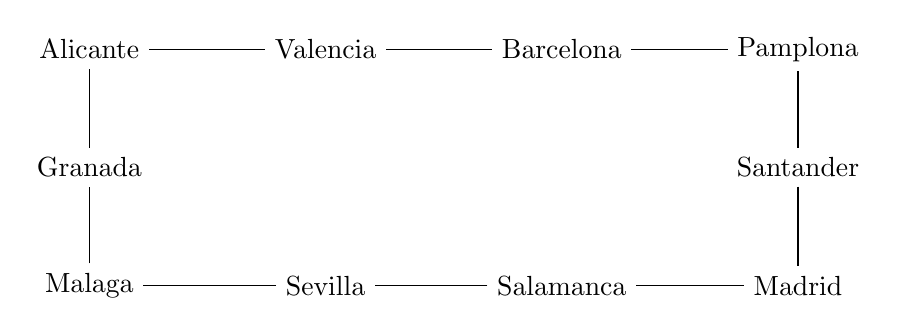
\begin{tikzpicture}
\node (a) at (0, 0) {Malaga};
\node (b) at (0, 1.5) {Granada};
\node (c) at (0, 3) {Alicante};
\node (d) at (3, 3) {Valencia};
\node (e) at (6, 3) {Barcelona};
\node (f) at (9, 3) {Pamplona};
\node (g) at (9, 1.5) {Santander};
\node (h) at (9, 0) {Madrid};
\node (i) at (6, 0) {Salamanca};
\node (j) at (3, 0) {Sevilla};
\draw (a)--(b)--(c)--(d)--(e)--(f)--(g)--(h)--(i)--(j)--(a);
\end{tikzpicture}
\caption{The fastest route around Spanish cities with the distances given in Table~\ref{tab:distance_matrix}.}
\label{fig:fastest_route_around_spannish_cities}
\end{center}
\end{figure}
\clearpage
